\documentclass{article}
\usepackage[a4paper]{geometry}
\usepackage{fullpage}
\usepackage{cleveref}
\usepackage{graphicx}
\usepackage{subcaption}
\usepackage[T1]{fontenc}
\usepackage[utf8]{inputenc}

\title{Rapport de projet de synthèse d'image}
\author{Thibaut Lepage, François Ripault}

\begin{document}

\maketitle

\section*{Introduction}

Ce rapport présente les éléments principaux du raytracer que nous avons
implémenté dans le cadre du cours du projet de synthèse d'image. Nous avons
implémenté quelques formes primitives: sphères, triangles et plans, et avons
ajouté un support pour les fichiers ".obj". Le modèle de lumière utilise un
modèle de Phong, qui gère les réflections et les lumières avec volume.

\section{Modèle de Phong}

Le modèle d'éclairage utilisé pour notre Raytracer est le modèle de réflection
de Phong. Il définit trois composantes pour la lumière, une composante
ambiante, une diffuse, et une spéculaire.
La \cref{phong} montre chacune des composantes de l'éclairage de Phong:

\begin{figure}[hb]
  \begin{subfigure}{0.45\textwidth}
    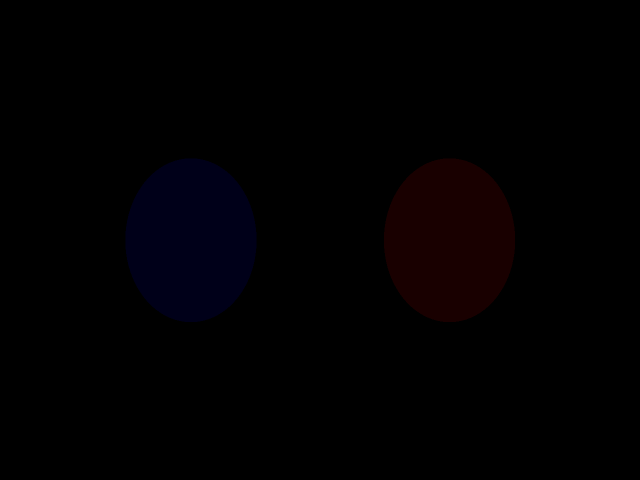
\includegraphics[width=1\textwidth]{images/phong1.png}
    \subcaption{Lumière ambiante}
  \end{subfigure}
  \begin{subfigure}{0.45\textwidth}
    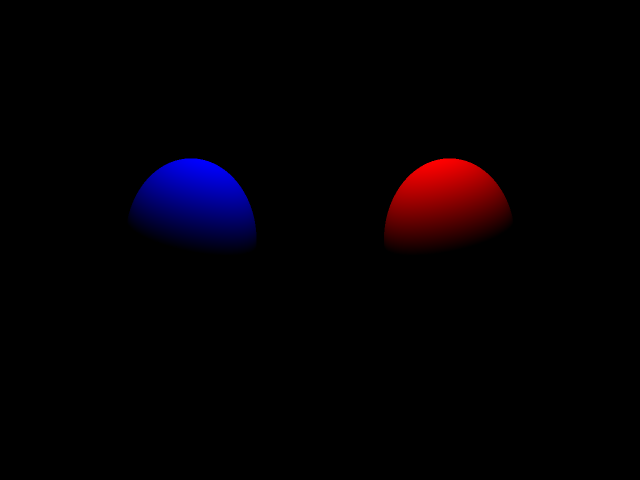
\includegraphics[width=1\textwidth]{images/phong2.png}
    \subcaption{Lumière diffuse}
  \end{subfigure}

  \begin{subfigure}{0.45\textwidth}
    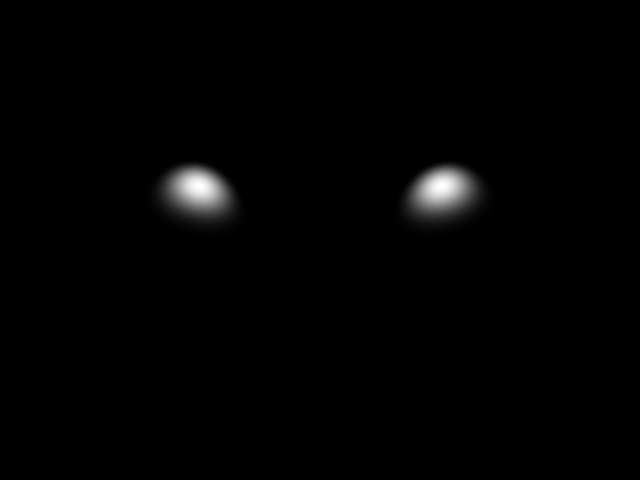
\includegraphics[width=1\textwidth]{images/phong3.png}
    \subcaption{Lumière spéculaire}
  \end{subfigure}
  \begin{subfigure}{0.45\textwidth}
    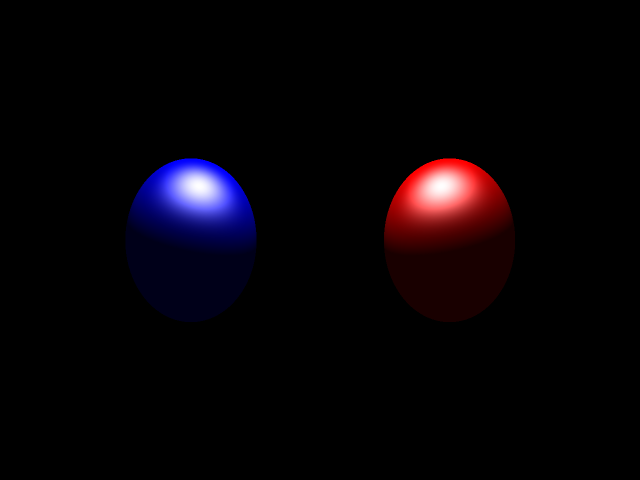
\includegraphics[width=1\textwidth]{images/phong4.png}
    \subcaption{Résultat final}
  \end{subfigure}
  \caption{Éclairage de Phong\label{phong}}
\end{figure}


\section{Réflection}
La réflection est implémentée simplement dans notre raytracer: lorsqu'un rayon
touche un objet, la fonction de lancer de rayon est appelée récursivement avec
le rayon réfléchi issu de l'intersection. La récursion s'arrête lorsque la
profondeur maximale de réflection est atteinte. La couleur résultante est ainsi
mélangée avec celle calculée à la surface de l'objet, selon le coefficient de
réflection de l'objet. La \cref{refl} détaille l'importance de la
réflection selon le coefficient associé.

\begin{figure}[hb]
  \begin{subfigure}{0.45\textwidth}
    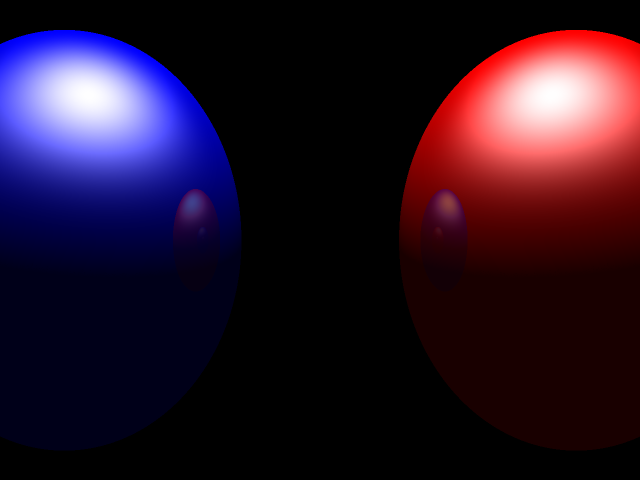
\includegraphics[width=1\textwidth]{images/refl025.png}
    \subcaption{Coefficient de 0.25}
  \end{subfigure}
  \begin{subfigure}{0.45\textwidth}
    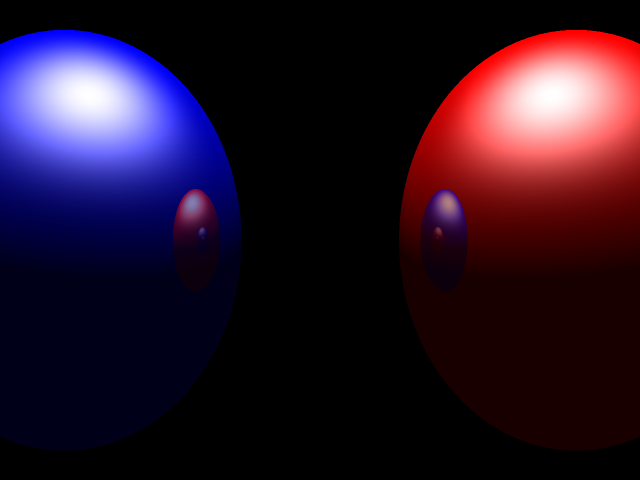
\includegraphics[width=1\textwidth]{images/refl05.png}
    \subcaption{Coefficient de 0.5}
  \end{subfigure}

  \begin{subfigure}{0.45\textwidth}
    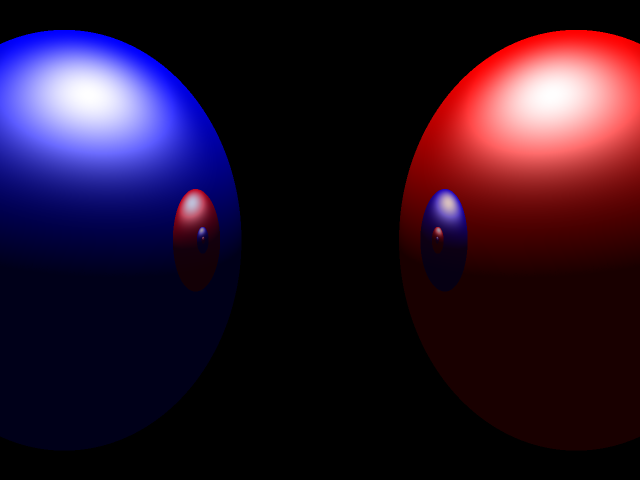
\includegraphics[width=1\textwidth]{images/refl075.png}
    \subcaption{Coefficient de 0.75}
  \end{subfigure}
  \begin{subfigure}{0.45\textwidth}
    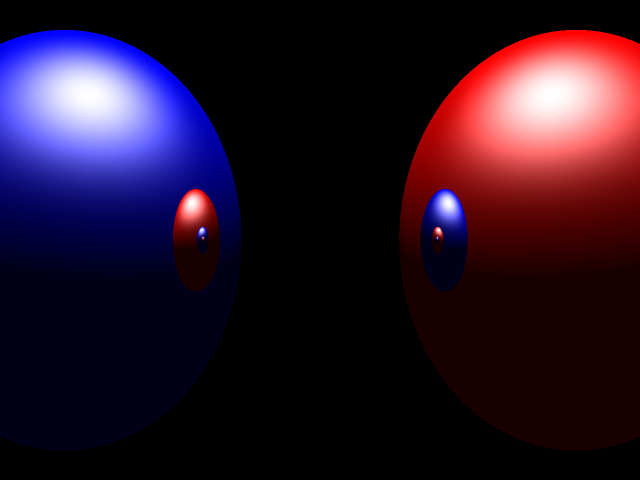
\includegraphics[width=1\textwidth]{images/refl1.png}
    \subcaption{Coefficient de 1}
  \end{subfigure}
  \caption{Réflection selon le coefficient\label{refl}}
\end{figure}

Car calculer la réflection sur un objet revient à lancer un rayon
supplémentaire, cela a un impact remarquable sur les performances. Afin
d'obtenir un résultat satisfaisant et suffisamment rapide à générer, la
profondeur maximale de réflection a été mise à 5.

\section{Lumières avec Volume}

Lorsque qu'un rayon atteint un objet, on vérifie que le point de l'objet est
bien éclairé: cela se fait en lançant un rayon du point d'intersection vers une
lumière, et en s'assurant qu'aucun autre objet est sur le chemin. Avec des
lumières simples, les ombres obtenues de cette manière sont dures, et ne
prennent pas en compte de la forme de l'objet pour la dureté de l'ombre.
Ceci est dû au fait que la lumière n'a pas de volume, et que donc, il n'y a
aucune gradation dans l'ombre de l'objet.

Afin d'obtenir de meilleures ombres, nous avons implémenté des lumières avec
volume. En gardant à l'esprit les performance, une lumière avec volume est en
fait une distribution uniforme de lumières sans volume sur une sphère d'un
rayon défini par l'utilisateur. Cela nous permet ainsi d'obtenir des ombres plus
douces, comme montré dans la \cref{light}.

\begin{figure}[hb]
  \begin{subfigure}{0.45\textwidth}
    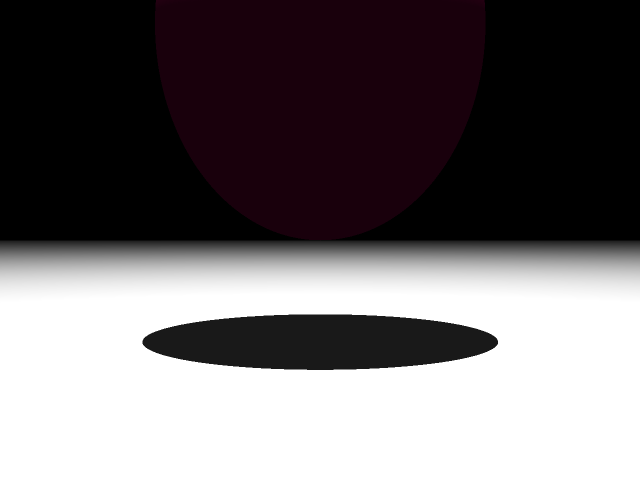
\includegraphics[width=1\textwidth]{images/samples0.png}
    \subcaption{Lumière sans échantillons}
  \end{subfigure}
  \begin{subfigure}{0.45\textwidth}
    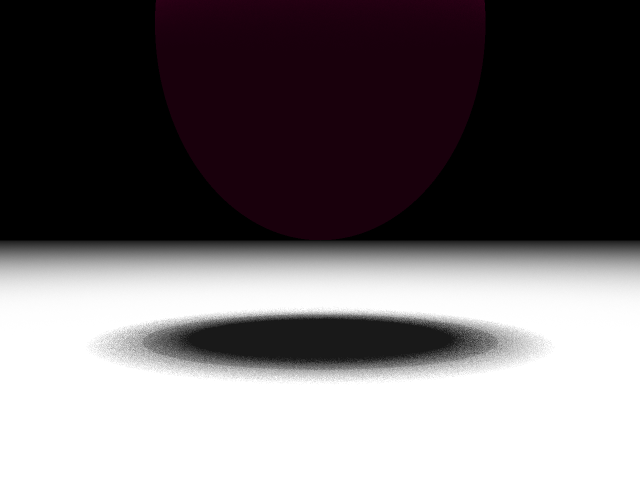
\includegraphics[width=1\textwidth]{images/samples10.png}
    \subcaption{Lumière avec 10 échantillons de rayon 1}
  \end{subfigure}

  \begin{subfigure}{0.45\textwidth}
    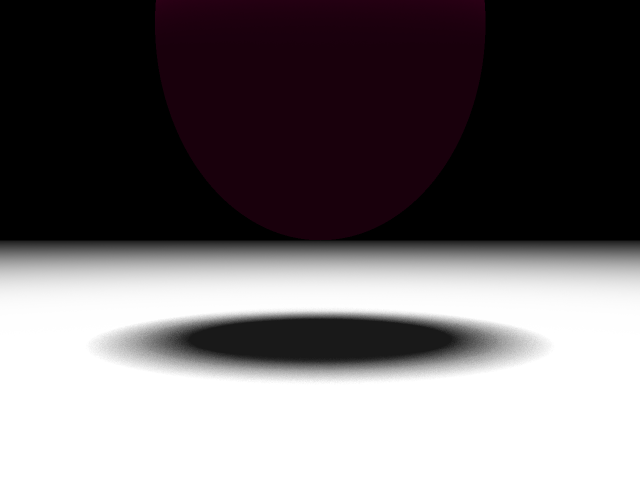
\includegraphics[width=1\textwidth]{images/samples50.png}
    \subcaption{Lumière avec 50 échantillons de rayon 1}
  \end{subfigure}
  \begin{subfigure}{0.45\textwidth}
    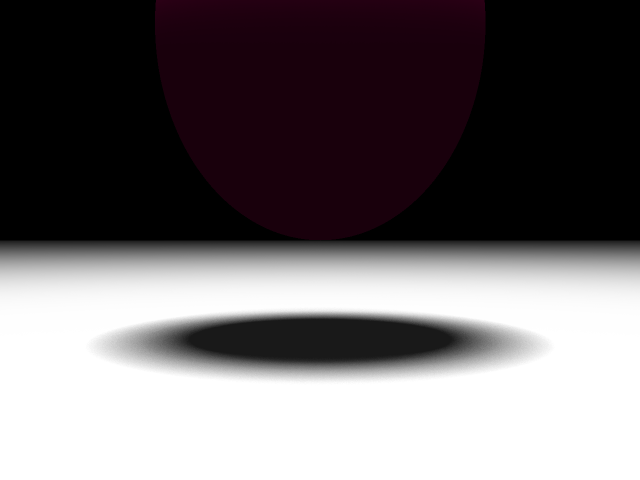
\includegraphics[width=1\textwidth]{images/samples100.png}
    \subcaption{Lumière avec 100 échantillons de rayon 1}
  \end{subfigure}

  \begin{subfigure}{0.45\textwidth}
    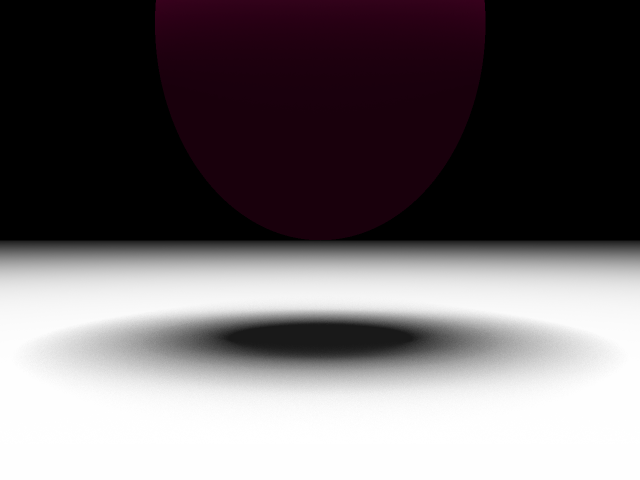
\includegraphics[width=1\textwidth]{images/samples100r2.png}
    \subcaption{Lumière avec 100 échantillons de rayon 2}
  \end{subfigure}
  \begin{subfigure}{0.45\textwidth}
    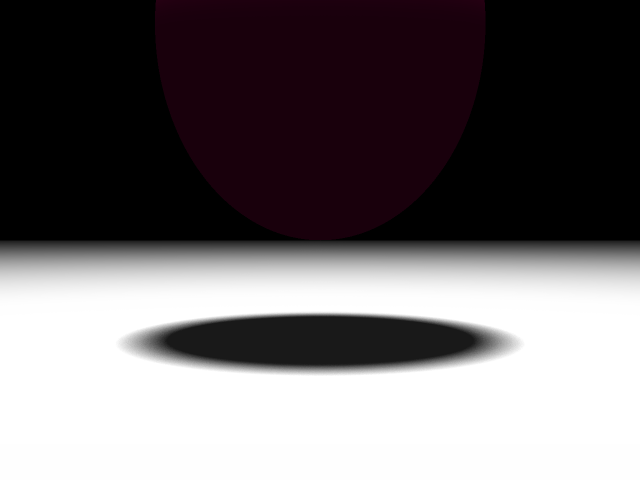
\includegraphics[width=1\textwidth]{images/samples100r05.png}
    \subcaption{Lumière avec 100 échantillons de rayon 0.5}
  \end{subfigure}
  \caption{Rendu de lumières avec volumes\label{light}}
\end{figure}

On constate que la la distribution aléatoire des point sur la sphère engendre
du bruit: celui ci est notamment visible sur l'exemple avec 10 échantillons.
Afin de réduire l'influence de ce bruit, on utilise un ``lissage'' de la
distribution de probabilité, en tirant des échantillons aléatoires dans une
zone bien définie. La \cref{smooth} décrit une telle méthode. L'image de
gauche contient une distribution purement aléatoire, et cela à pour défaut de
laisser certaines zone de l'image vide. En contraignant le tirage
d'échantillons dans une grille, on obtient une distribution beaucoup plus
uniforme, ce qui réduit le bruit lors du rendu d'une ombre, comme dans l'image
de droite.

\begin{figure}[h]
\begin{center}
  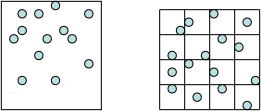
\includegraphics{images/smoothing.png}
  \caption{Exemple de lissage aléatoire\label{smooth}}
\end{center}
\end{figure}


\section{Chargement d'objet et KDTree}

Afin de proposer à l'utilisateur de rendre des formes plus complexes, nous
gérons le chargement de fichiers ".obj" dans notre raytracer. Nous utilisons
pour cela la bibliothèque \texttt{tinyobjloader} qui nous parse un fichier, et
nous traduisons leur format de donnée de cette bibliothèque vers notre
représentation.

Afin d'accélérer le rendu, l'ensemble des triangles d'un objet sont représentés
sous la forme d'un KDTree. C'est un arbre binaire pour lequel, à chaque niveau
de l'arbre, les objets sont séparés selon un axe (x, y, ou z). Pour trier les
objets, on se base sur la composante du centre des objets, et les objets sont
triés et séparés selon la médiane. Cela nous permet d'obtenir un arbre
équilibré.

Chaque noeud de l'arbre possède une boite englobante qui contient tous les
triangles du sous arbre, ainsi, si un rayon n'intersecte pas cette boite
englobante, cela implique qu'ils n'intersecte aucun des triangles du
sous-arbre. Cela nous permet de gagner en performance lors du rendu des objets.

De la même manière, l'ensemble des formes contenues dans une scène est
représentée également sous la forme d'un KDTree. La \cref{obj} montre
quelques objets chargés de cette manière.

\begin{figure}[hb]
  \begin{subfigure}{0.45\textwidth}
    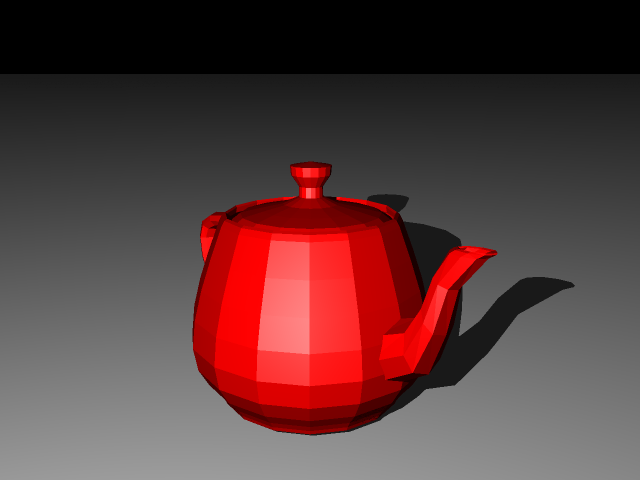
\includegraphics[width=1\textwidth]{images/obj1.png}
    \subcaption{Rendu d'une théière}
  \end{subfigure}
  \begin{subfigure}{0.45\textwidth}
    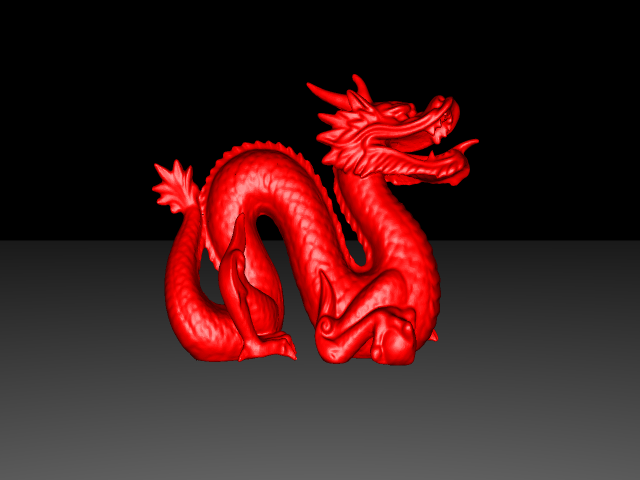
\includegraphics[width=1\textwidth]{images/obj2.png}
    \subcaption{Rendu d'un dragon}
  \end{subfigure}

  \begin{subfigure}{0.45\textwidth}
    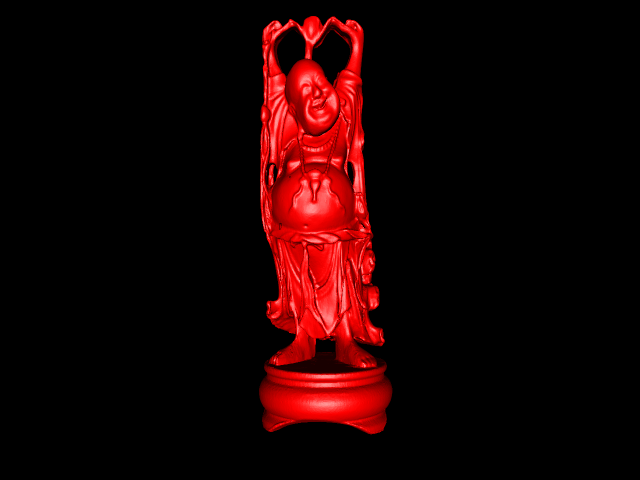
\includegraphics[width=1\textwidth]{images/obj3.png}
    \subcaption{Rendu d'un Bouddha}
  \end{subfigure}
  \caption{Rendu de différents objets\label{obj}}
\end{figure}

\section{Interpolation de normales}

On remarque dans les images précédentes que l'éclairage est fortement impacté
par le nombre de polygones dans l'objet. En effet, la lumière ne prend en
compte que le triangle courant pour le rendu, et non le contexte du triangle.
Ainsi, si l'on désire rendre une surface courbe, cela a pour conséquence
d'avoir un mauvais rendu.

Afin de parer à ce problème, le format ".obj" définit des normales au sommets,
qui sont en fait la somme des normales des triangles associés à un sommet. A
partir de ces normales au sommets, il est ainsi possible d'interpoler la
normale en un point du triangle, en fonction de sa proximité aux sommets de ce
triangle. La \cref{normal} affiche les normales de l'objet, avec et sans
interpolation, et le rendu obtenu. La couleur décrit la direction du vecteur
normal: le rouge représente l'axe x, le vert l'axe y, et le bleu l'axe z.

\begin{figure}[hb]
  \begin{subfigure}{0.45\textwidth}
    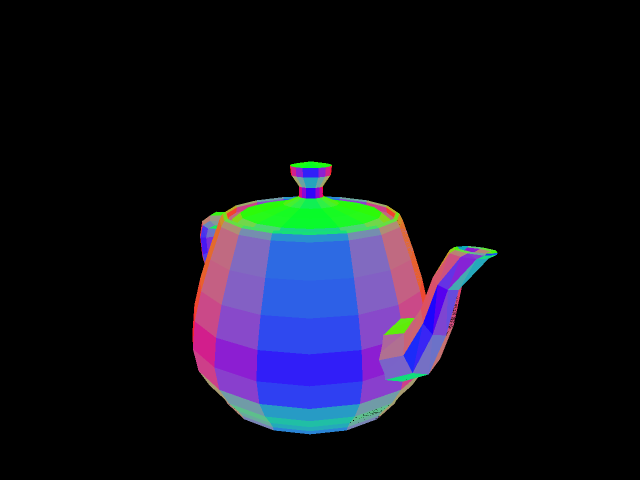
\includegraphics[width=1\textwidth]{images/normal1.png}
    \subcaption{Normales sur la théière}
  \end{subfigure}
  \begin{subfigure}{0.45\textwidth}
    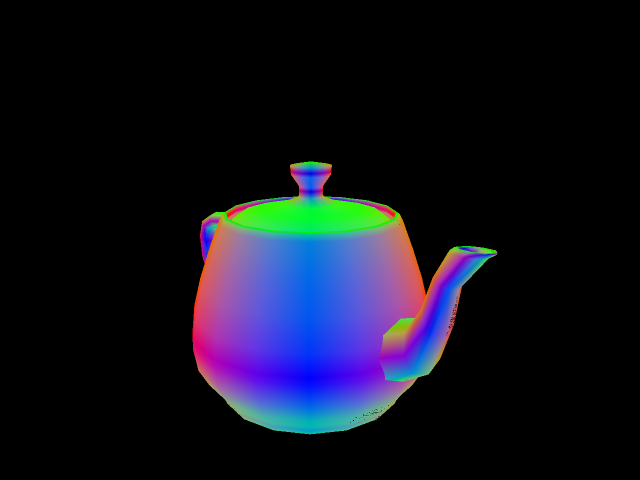
\includegraphics[width=1\textwidth]{images/normal2.png}
    \subcaption{Normales interpolées sur la théière}
  \end{subfigure}

  \begin{subfigure}{0.45\textwidth}
    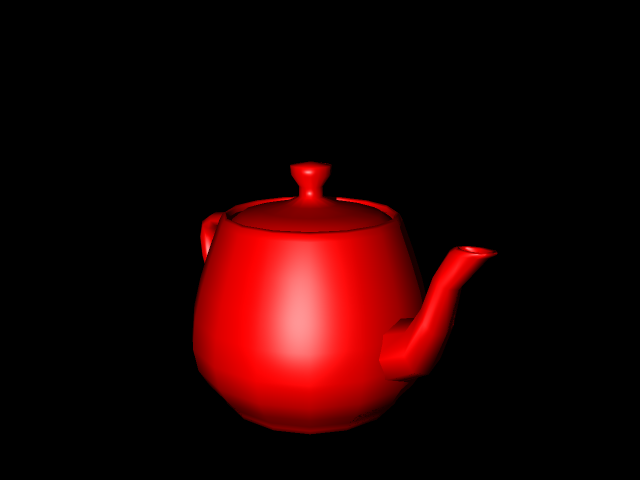
\includegraphics[width=1\textwidth]{images/nres1.png}
    \subcaption{Résultat final}
  \end{subfigure}

  \caption{Résultats de l'interpolation de normales\label{normal}}
\end{figure}

\section{Anti-crénelage}

Lors du rendu des images, on constate un effet de crénelage qui est du à au
fait que un pixel ne décrit pas fidèlement la couleur dans une zone de l'image:
si un rayon est proche de la frontière d'un objet, il retournera la couleur de
cet objet, sans prendre en compte le fait que il est situé à l'extrémité de
l'objet. Afin de parer à ce problème, on utilise la technique du
``supersampling'', qui consiste à lancer plusieurs rayon pour un même pixel,
comme montré dans la \cref{super}.

Pour cela, on augmente la taille de l'image selon un facteur donné, afin de
faire correspondre un ensemble de pixels à le pixel d'origine, pour avoir une
couleur décrivant plus précisément la région affichée.

\begin{figure}
  \begin{center}
  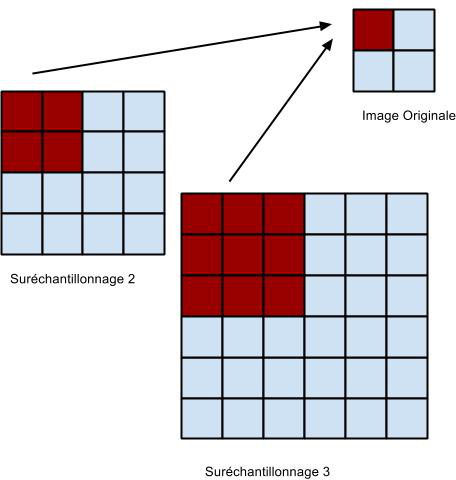
\includegraphics[width=0.5\textwidth]{images/supersampling.jpg}
  \end{center}
  \caption{Méthode de suréchantillonnage\label{super}}
\end{figure}

Avec cette méthode, il est possible d'obtenir de meilleurs résultats sur les images générées, comme dans \cref{superresults}

\begin{figure}[hb]
  \begin{subfigure}{0.45\textwidth}
    
\includegraphics[width=1\textwidth]{images/super1.png}
    \subcaption{Suréchantillonnage facteur 1}
  \end{subfigure}
  \begin{subfigure}{0.45\textwidth}
    
\includegraphics[width=1\textwidth]{images/super2.png}
    \subcaption{Suréchantillonnage facteur 2}
  \end{subfigure}

  \begin{subfigure}{0.45\textwidth}
    
\includegraphics[width=1\textwidth]{images/super3.png}
    \subcaption{Suréchantillonnage facteur 3}
  \end{subfigure}
  \begin{subfigure}{0.45\textwidth}
    
\includegraphics[width=1\textwidth]{images/super4.png}
    \subcaption{Suréchantillonnage facteur 4}
  \end{subfigure}
  \caption{Rendu d'une sphère selon différentes valeurs de suréchantillonnage\label{superresults}}
\end{figure}

\section{Textures}

Pour représenter des objets aux textures plus variées qu'une simple couleur
unie, on a choisi d'associer à chaque objet un foncteur qui, à partir de deux
coordonnées dans un plan virtuel infini (la texture), retourne la couleur en
ce point.

\subsection{Textures bitmap}

Dans le cas des textures bitmap, c'est-à-dire directement chargées depuis une
image matricielle, le foncteur renvoie simplement la couleur du pixel demandé
sur l'image.

\subsection{Textures procédurales}

\subsubsection{Formes standards}

Le foncteur est défini dans le fichier de description d'une scène comme une
liste de couleurs associées à des contraintes sur un plan. On génère une
\emph{closure} à partir de ces contraintes, et chaque forme (sphère, triangle,
etc.) possède une méthode permettant d'associer à l'un des points de sa
surface (en 3D) un point sur le plan de texture (en 2D) avec respect des
distances.

\subsubsection{Formes importées depuis un fichier \texttt{.obj}}

Les textures doivent être définies en même temps que l'objet lui-même (à
l'aide d'un fichier \texttt{.mtl}), par facette, et la couleur en un point est
récupérée en utilisant le fait que les composants d'un Objet sont des formes
standards.

\section{Exemples de rendus}

\end{document}
